% fancytikzposter.tex, version 2.1
% Original template created by Elena Botoeva [botoeva@inf.unibz.it], June 2012
% 
% This file is distributed under the Creative Commons Attribution-NonCommercial 2.0
% Generic (CC BY-NC 2.0) license
% http://creativecommons.org/licenses/by-nc/2.0/ 


\documentclass{a0poster}

\usepackage{fancytikzposter} 

%%%%% --------- Change here if you want ---------- %%%%%
%% margin for the geometry package, must be changed before using the geometry package
%% default value is 4cm
% \setmargin{4}

%% the space between the blocks
%% default value is 2cm
\setblockspacing{1}

%% the height of the title stripe in block nodes, decrease it to save space
%% default value is 3cm
% \setblocktitleheight{3}

%% the number of columns in the poster, possible values 2,3
%% default value is 2
% \setcolumnnumber{3}

%% the space between two or more groups of authors from different institutions
%% used in \maketitle
% \setinstituteshift{10}

%% which template to use
%% N1 simple, standard look, with a colored background and gray boxes
%% N2 board with nodes
%% N3 another standard look
%% N4 envelope-like look
%% N5 with a wave-like head, original idea taken from
%%%% http://fc09.deviantart.net/fs71/f/2010/322/1/1/scientific_poster_by_nabuy-d333ria.jpg
%\usetemplate{5}

%% components of the templates
%% (the maximal possible numbers are mentioned as the parameters)
% \usecolortemplate{4}
% \usebackgroundtemplate{5}
% \usetitletemplate{3}
% \useblocknodetemplate{5}
% \useplainblocktemplate{4}
% \useinnerblocktemplate{2}


%% the height of the head drawing on top 
%% applicable to templates N3, 4 and 5
% \setheaddrawingheight{14}


%% change the basic colors
%\definecolor{myblue}{HTML}{008888} 
%\setfirstcolor{myblue}% default 116699
%\setsecondcolor{gray!80!}% default CCCCCC
%\setthirdcolor{red!80!black}% default 991111

%% change the more specific colors
% \setbackgrounddarkcolor{colorone!70!black}
% \setbackgroundlightcolor{colorone!70!}
% \settitletextcolor{textcolor}
% \settitlefillcolor{white}
% \settitledrawcolor{colortwo}
% \setblocktextcolor{textcolor}
% \setblockfillcolor{white}
% \setblocktitletextcolor{colorone}
% \setblocktitlefillcolor{colortwo} %the color of the border
% \setplainblocktextcolor{textcolor}
% \setplainblockfillcolor{colorthree!40!}
% \setplainblocktitletextcolor{textcolor}
% \setplainblocktitlefillcolor{colorthree!60!}
% \setinnerblocktextcolor{textcolor}
% \setinnerblockfillcolor{white}
% \setinnerblocktitletextcolor{white}
% \setinnerblocktitlefillcolor{colorthree}




%%% size of the document and the margins
%% A0
% \usepackage[margin=\margin cm, paperwidth=118.9cm, paperheight=84.1cm]{geometry} 
\usepackage[margin=\margin cm, paperwidth=84.1cm, paperheight=118.9cm]{geometry}
%% B1
% \usepackage[margin=\margin cm, paperwidth=70cm, paperheight=100cm]{geometry}



%% changing the fonts
\usepackage{cmbright}
%\usepackage[default]{cantarell}
%\usepackage{avant}
%\usepackage[math]{iwona}
\usepackage[math]{kurier}
\usepackage[T1]{fontenc}


%% add your packages here
%\usepackage{hyperref}  % % DISABILITATO I VIRTUAL REF


% % % DAN ADDED
\newtheorem{thm3}{Proposition}

% % % END DAN ADDED

\title{Minimum-energy bandwidth management for QoS live migration of virtual machines} %Networking-Computing resource allocation for Hard Real-Time Green Cloud applications}
%\author{Elena Botoeva\\
%  KRDB Research Centre, Free University of Bozen-Bolzano, Italy\\
%  \texttt{botoeva@inf.unibz.it}
%}
\author{D. Amendola; N. Cordeschi; E. Baccarelli\\ %\vspace{20pt}
	danilo.amendola@uniroma1.it - Computer Networks - 2015, \\ 
	poster presentation at ComSoc Summer School '16}

\begin{document}

%%%%% ---------- the background picture ---------- %%%%%
%% to change it modify the macro \BackgroundPicture
\ClearShipoutPicture
\AddToShipoutPicture{\BackgroundPicture}

\noindent % to have the picture right in the center
\begin{tikzpicture}
  \initializesizeandshifts
  % \setxshift{15}
  % \setyshift{2}


  %% the title block, #1 - shift, the default value is (0,0), #2 - width, #3 - scale
  %% the alias of the title block is `title', so we can refer to its boundaries later
  \ifthenelse{\equal{\template}{1}}{ 
    \titleblock{47}{1}
  }{
    \titleblock{47}{1.5}
  }

  %% a logo can be added to the title block
  %% #1 - anchor relative to the title block, #2 - shift, #3 - width, #3 - file name
   \ifthenelse{\equal{\template}{2}}{ 
     \addlogo[south west]{(2,0)}{6cm}{unibz_b.png}
   }{
     \addlogo[south west]{(1,0.5)}{6cm}{logos/ieee-comsoc.png} 
     \addlogo[south west]{(41,1)}{7cm}{logos/ieee.jpg}
   }


  %% a block node, with the specified position (optional), title and the content
  %% #1 - where (optional), #2 - title, #3 - text
  %%%%%%%%%% ------------------------------------------ %%%%%%%%%%
  \blocknode{Abstract}
  {%\emph{
  	Live virtual machine (VM) migration aims at enabling the dynamic balanced use of the networking/computing physical resources of virtualized datacenters, so to lead to reduced energy consumption. However, the bandwidth consumption and latency of current state-of-the-art live VM migration techniques still reduce the experienced benefits to much less than their potential. Motivated by this consideration, in this paper, we analytically characterize, prototype in software and test through field trials the optimal bandwidth manager for intra-datacenter live migration of VMs. The goal is the minimization of the migration-induced communication energy under service level agreement (SLA)-induced \emph{hard} constraints on the total migration time, downtime, slowdown of the migrating applications and overall available bandwidth. For this purpose, after recognizing that the resulting (nonconvex) optimization problem is an instance of Geometric Programming, we solve it by resorting to suitably developed \textit{adaptive} version of the so-called primal-dual gradient-based iterations and, then, we analytically characterize its feasibility conditions. Hence, we prototype the resulting bandwidth manager atop an intra-datacenter wired test-bed, and, then, test and compare its energy performance through extensive field trials. The carried out field trials point out that: (i) the \textit{energy savings} attained by the proposed bandwidth manager over the state-of-the-art ones currently utilized by Xen, KVM and VMware hypervisors are \textit{over} 40\% and \textit{approach} 66\% under strict QoS constraints;  (ii) the proposed bandwidth manager is capable to \textit{quickly adapt} to the abrupt changes possibly experienced by the dirty rates of the running applications and/or the round trip times of the utilized (possibly, congested) TCP/IP connections; and,  (iii) its actual implementation may be carried out in a \emph{distributed} and \emph{scalable} way, and it consumes \textit{less} than 1.5\% of the CPU computing power per migrated VM.
  		%}
  }
  
  \vspace{80pt}
  \blocknode%
  {Introduction and Architecture}%
  { 
  	%The goal of the Green Cloud Computing is to develop models and techniques for the integrated management of computing-communication virtualized platforms, so as to provide QoS, robustness and energy efficiency. The resulting challenge is to minimize the energy usage and still meet the QoS requirements of the supported applications. About the QoS support,  an energy-saving \emph{joint} allocation of both networking and computing resources hosted in the Cloud is needed. This is the focus of this paper, where the contrasting objectives of minimizing \emph{both} networking  and computing energies in \emph{real-time} applications running on top of virtualized Clouds are cast in the form of a suitable \emph{constrained} optimization problem.
	\begin{tikzfigure}[Reference VNetDC architecture for intra-datacenter live VM migration. Continue (resp., dotted) arrowed lines denote end-to-end TCP connections conveying migration (resp., application) traffic. Dashed-dotted arrowed lines denote signalling flows for implementing the resource profiling and migration plan. APP: application; VMM: virtual machine manager; OS: operating system; HW: networking/computing hardware; EVS: external virtual switch; VNIC: virtual network interface card; NIC: physical network interface card; NAS: network-attached storage.]
	%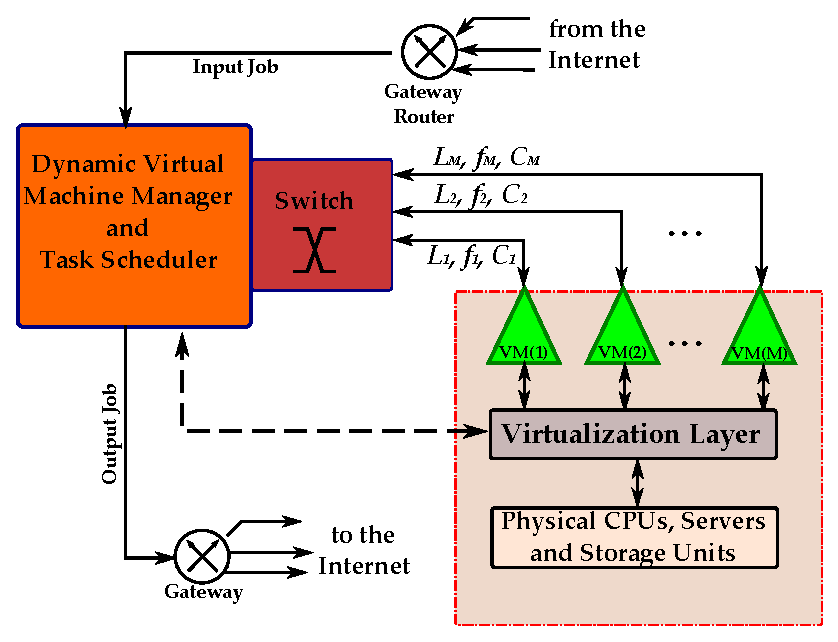
\includegraphics[width=0.7\columnwidth]{images/Modello.eps}
	\includegraphics[width=0.55\columnwidth]{images/Fig1}
	\label{fig:1}
	\end{tikzfigure}
  }

  %% by default, the position of the new block node is right below the previous
  %% block node, stored in (currenty)
  %% box is the alias of the previous block, so we can refer to its boundaries

  %%%%%%%%%% ------------------------------------------ %%%%%%%%%%
  \blocknode{Problem setup and optimal resource allocation}%
  {
  	
  	Let $R$ $(Mb/s)$ be the transmission rate used during the third and fourth stages for migrating the VM, that is, the migration bandwidth. Since, by definition, only ${T_{IP}}$ and ${T_{SC}}$ depend
  	\begin{tikzfigure}[Time-chart of the PeCM technique.]
  	\centering
  	\includegraphics[width=0.65\columnwidth]{images/Fig2}
  	%\caption{Time-chart of the PeCM technique.}
  	\label{fig:2}
  	\end{tikzfigure}
  	on $R$, while all the remaining migration times in Eqs. \eqref{eqn_1} and \eqref{eqn_2} play the role of constant parameters, in the sequel, we focus on the evaluation of the (already defined) stop-and-copy time ${T_{SC}}$ and the resulting memory migration time $T_{MMT}$, which is defined as in:
  	\begin{equation}
  	\label{eqn_3}
  	T_{MMT}~ \equiv~ T_{MMT}(R) ~\triangleq~ T_{IP}(R)+T_{SC}(R).
  	\end{equation}
  	
  }
  
  \blocknode{BroadcomLab Research Group}
  {
  \textit{\textbf{Keyword}}: Mobile Cloud Computing; Vehicular Cloud Computing; Big Data; Green Data Center; Communication and Computing Engineering in Cloud and Big Data; LTE; Next Generation ADSL.
  
  	  	%
  	  	\begin{minipage}[b]{0.77 \linewidth}
  	  	\LARGE BroadcomLab \\
  		\large
  		DIET Dept. at Sapienza University of Rome\\
  		First floor, room 101 - Via Eudossiana, 18, Rome (Italy)\\
  		phone: 0039 06 4458 5 366 - \textit{broadcom.diet.uniroma1.it}
  		\end{minipage}
  		%
  		\begin{minipage}[b]{0.2 \linewidth}
  		\begin{tikzfigure}
  		
\includegraphics[height=5.5cm]{logos/logosap.jpg}
  		\end{tikzfigure}
  		\end{minipage}
  		
%  	Laboratorio di Sistemi di Comunicazione a Banda Larga (BroadcomLab)
%  	Temi: le attività di ricerca, progettazione e sviluppo del laboratorio includono:(i) ideazione, progettazione, sviluppo validazione e prototipazione di piattaforme integrate di comunicazione/calcolo per il supporto di applicazioni di Mobile Cloud Computing, Vehicular Cloud Computing e Big Data; (ii) ideazione, progettazione e sviluppo di Green Data Center su infrastrutture di rete a banda larga e larghissima; (iii) communication and computing engineering per sistemi Cloud e Big Data; (iv) progettazione e sviluppo di sistemi di comunicazione a banda larga e larghissima di tipo "radio" (LTE-A) e "cablato" (next generation ADSL).
%  	Strumentazione: workstation e server per applicazioni networked Cloud.
%  	Tool di simulazione: Xen, VMWare, Matlab, OMNET++, Compilatori C/C++.
  	}
%  \vspace{3cm}
%  \blocknode{Authors}
%  {
%  	
%  	\begin{minipage}[t]{0.23 \linewidth}
%  	\centering
%  	Nicola Cordeschi\\
%  	Sapienza University of Rome
%  	\begin{tikzfigure}[]
%  	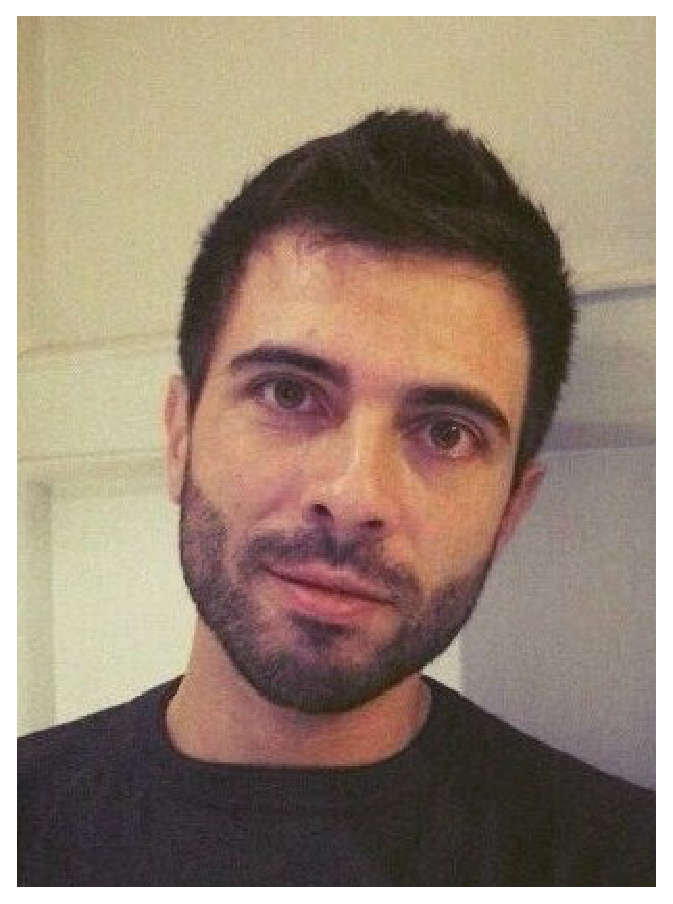
\includegraphics[height=7cm]{authors/nicola_cordeschi.eps} %width=0.7\columnwidth
%  	\end{tikzfigure}
%  	\end{minipage}
%  	%
%  	\begin{minipage}[t]{0.23 \linewidth}
% 	\centering
%  	Danilo Amendola\\
%  	Sapienza University of Rome
%  	\begin{tikzfigure}[]
%  	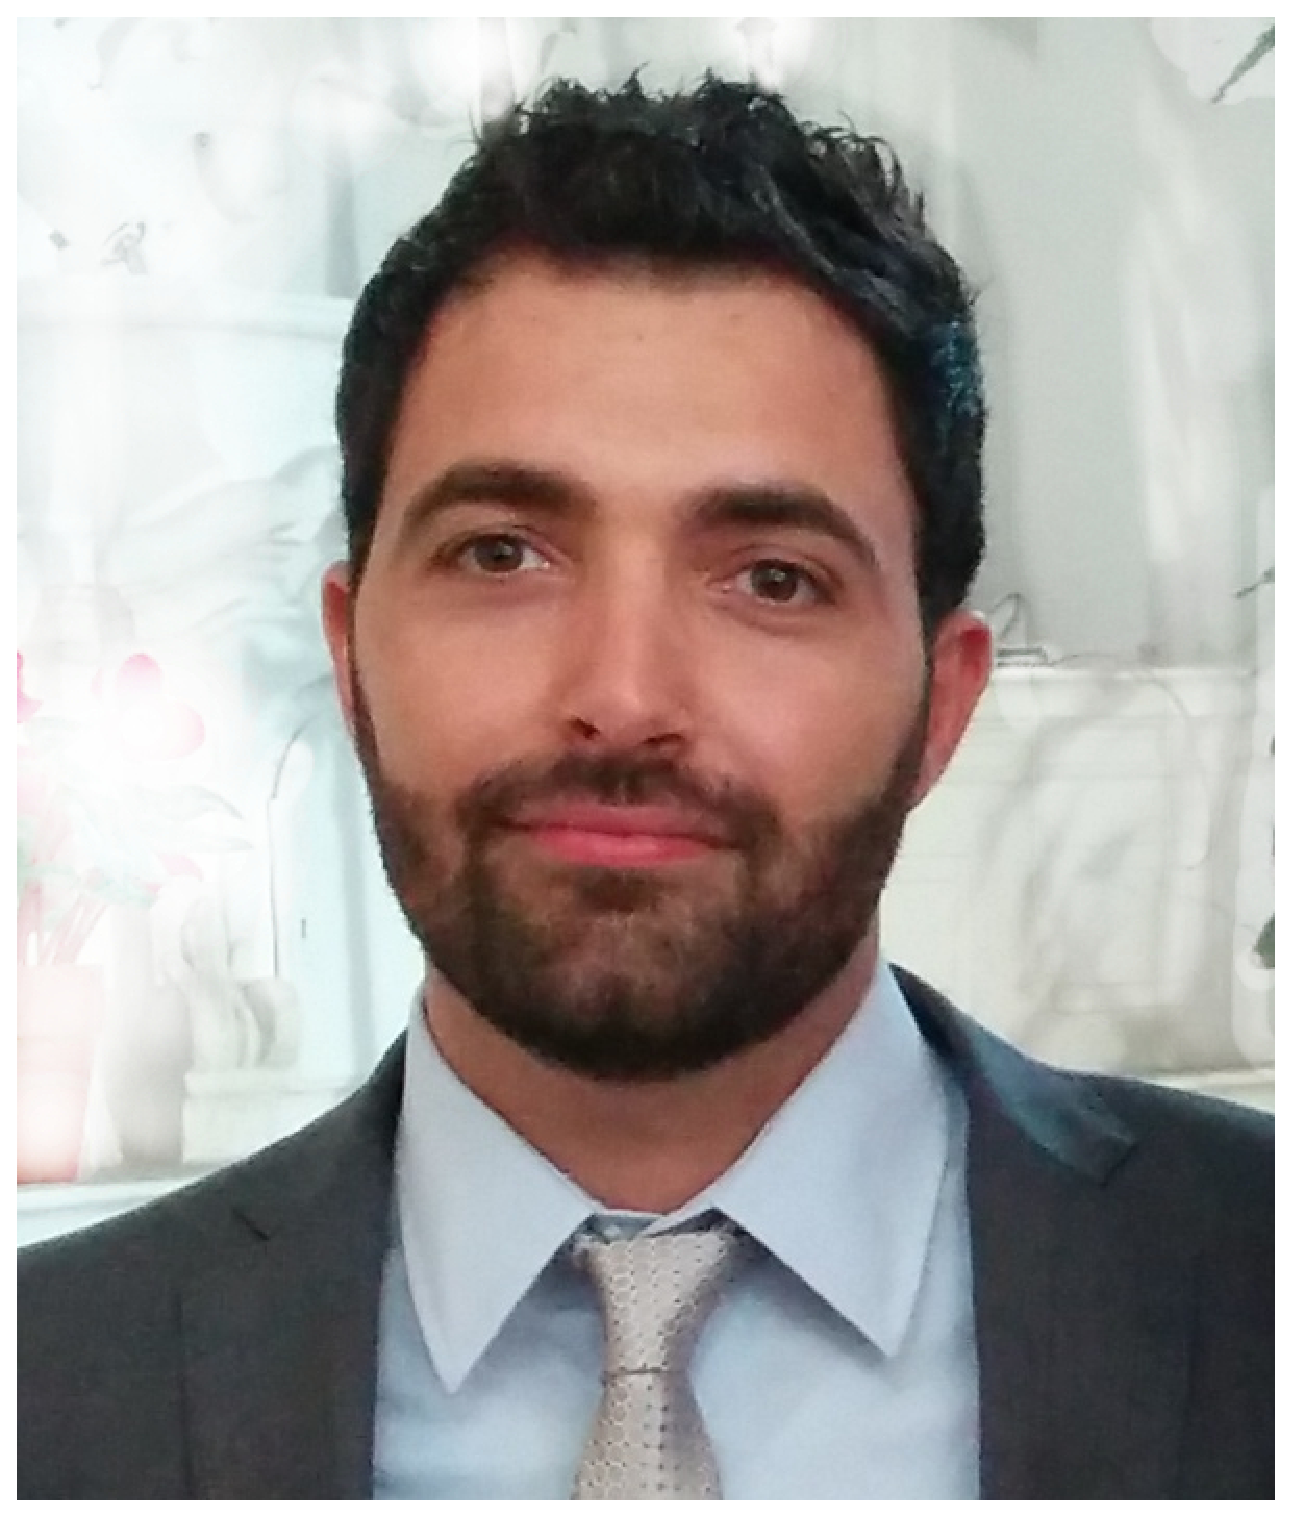
\includegraphics[height=7cm]{authors/danilo_amendola.eps}
%  	\end{tikzfigure}
%  	\end{minipage}
%  	%
%  	\begin{minipage}[t]{0.23 \linewidth}
%	\centering
%  	Floriano De Rango\\
%  	University of Calabria
%  	\begin{tikzfigure}[]
%  	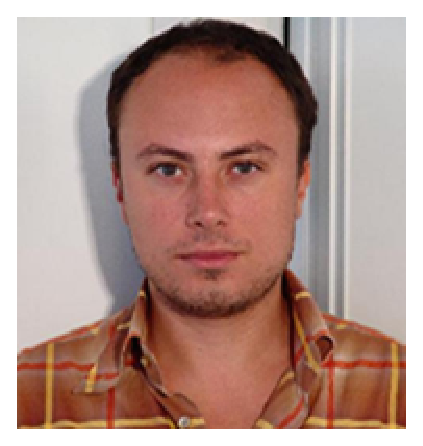
\includegraphics[height=7cm]{authors/floriano_derango.eps}
%  	\end{tikzfigure}
%  	\end{minipage}
%  	%
%  	\begin{minipage}[t]{0.23 \linewidth}
%  	\centering
%  	Enzo Baccarelli\\
%  	Sapienza University of Rome
%  	\begin{tikzfigure}[]
%  	
\includegraphics[height=7cm]{authors/enzo_baccarelli.eps}
%  	\end{tikzfigure}
%  	\end{minipage}
%   }
 	
	\startsecondcolumn

  %%%%%%%%%% ------------------------------------------ %%%%%%%%%%
  %\blocknodew[($(currenty)-(3.5,0)$)]{30}{Variable Width Block Nodes} %
  \blocknode %
  {Results on the tracking capabilities under connection phenomena} %
  {
  	
  	
  	\vspace{-30pt}
  		\begin{minipage}[t]{0.5 \linewidth}
  		\flushleft
  		\begin{tikzfigure}[Time evolutions (in the \textit{n} index) of the energy consumption of the proposed bandwidth manager at: $\widehat{R}= 900$ $(Mb/s)$, ${M_{0}=512}$ $(Mb)$, $\beta=1.15$, $\Delta_{MMT}=13.5$ $(s)$,  $\Delta_{SC}=0.6$ $(s)$, $\widetilde{I}_{MAX}=3$, and $\gamma=100$ for the application scenario of Section \ref{sec:7.3}.  (a) Case of time-varying ${\overline{\textit{w}}}$; (b) Case of time-varying $K_{0}$.]
  		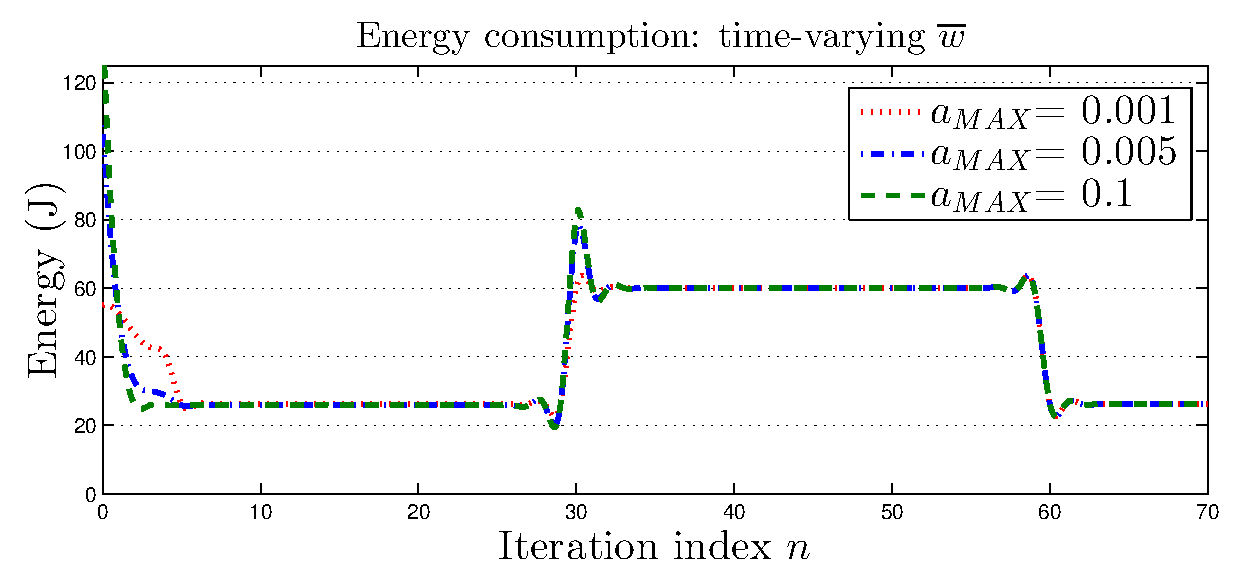
\includegraphics[width=1\columnwidth]{images/Fig3a} \\
  		 %\label{fig:3a}
  		 \vspace{10pt}
  		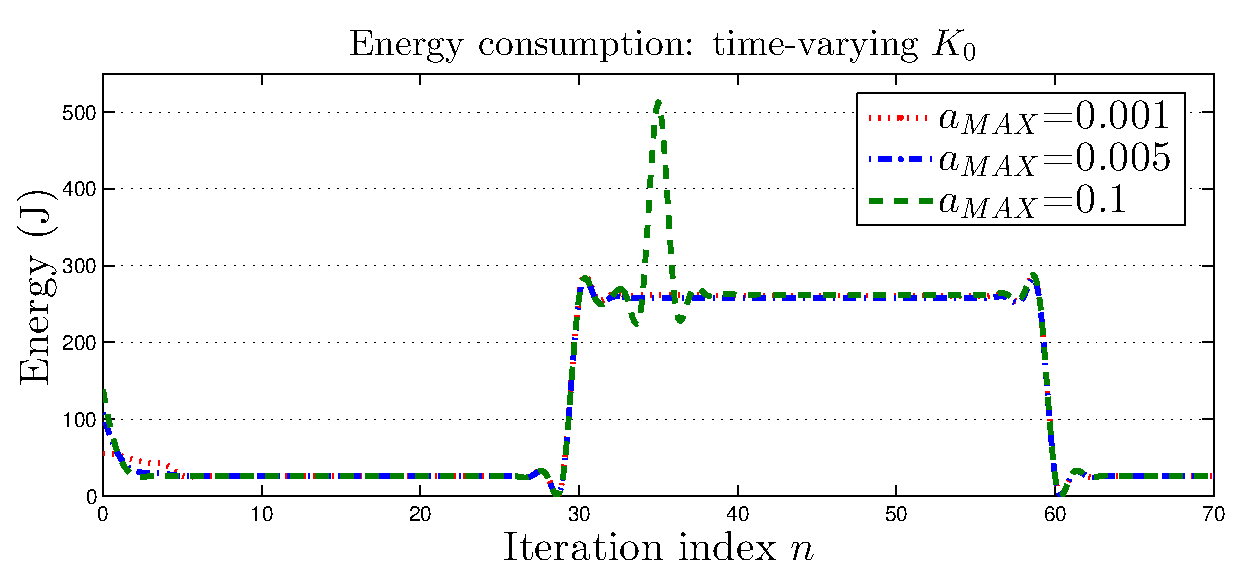
\includegraphics[width=1\columnwidth]{images/Fig3b}\label{fig:3}
  		\end{tikzfigure}
  		\end{minipage}
  		\begin{minipage}[t]{0.5 \linewidth}
%  		\begin{tikzfigure}[...]
%  		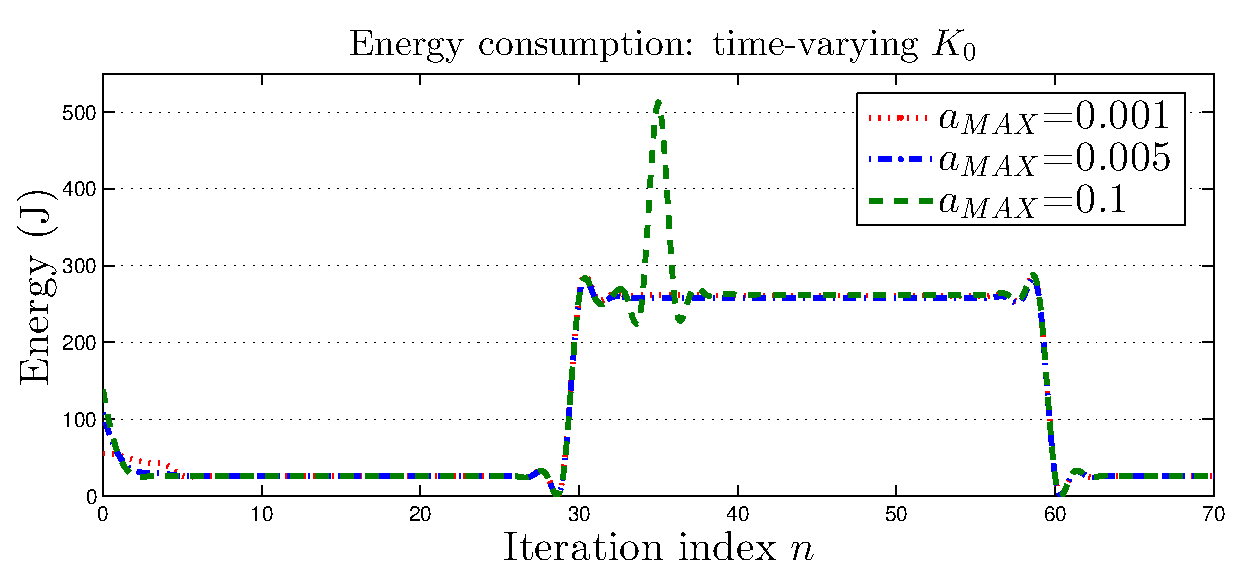
\includegraphics[width=0.8\columnwidth]{images/Fig3b.eps}\label{fig:3b}
%  		\end{tikzfigure}
  		\end{minipage}
	}

     %%%%%%%%%% ------------------------------------------ %%%%%%%%%%
     %\blocknodew[($(currenty)-(3.5,0)$)]{30}{Variable Width Block Nodes} %
     \blocknode %
     {Results Imax } %
     {
     	To evaluate the effect on  $\mathcal{E}_{tot}^*$  of the networking powers, we have set: $T_t=500$ $(ms)$, $C_{max}=150$ $(Mbit/s)$,
     	$L_t=10$ $(Mbit)$, $k_e=0.05 (mJ)/(MHz)^2$, $f_i^{max}=100$ $(Mbit/s)$, $f_i^{0}=0$ $(Mbit/s)$, $\mathcal{E}_i^{max}=1$ $(mJ)$, $\Delta(i)=1$ $(s)$.
     	We have evaluated $\mathcal{E}_{tot}^*$  (\emph{Joule}) for the following three network scenarios: \emph{i)} $P_i^{net}=0$ $(mW)$ (i.e., no communication costs); \emph{ii)} $P_i^{net}=1$ $(mW)$ (i.e., homogeneous communication costs); and, \emph{iii)} $P_i^{net}=1+0.25(i-1)$ $(mW)$, for $i=1,\ldots,M$ (i.e., heterogeneous communication costs).
     	
     	\vspace{-30pt}
     	\begin{minipage}[t]{0.5 \linewidth}
     	\flushleft
     	\begin{tikzfigure}[Time evolutions (in the \textit{n} index) of the energy consumption of the proposed bandwidth manager at: $\widehat{R}= 900$ $(Mb/s)$, ${M_{0}=512}$ $(Mb)$, $\beta=1.15$, $\Delta_{MMT}=13.5$ $(s)$,  $\Delta_{SC}=0.6$ $(s)$, $\widetilde{I}_{MAX}=3$, and $\gamma=100$ for the application scenario of Section \ref{sec:7.3}.  (a) Case of time-varying ${\overline{\textit{w}}}$; (b) Case of time-varying $K_{0}$.]
     	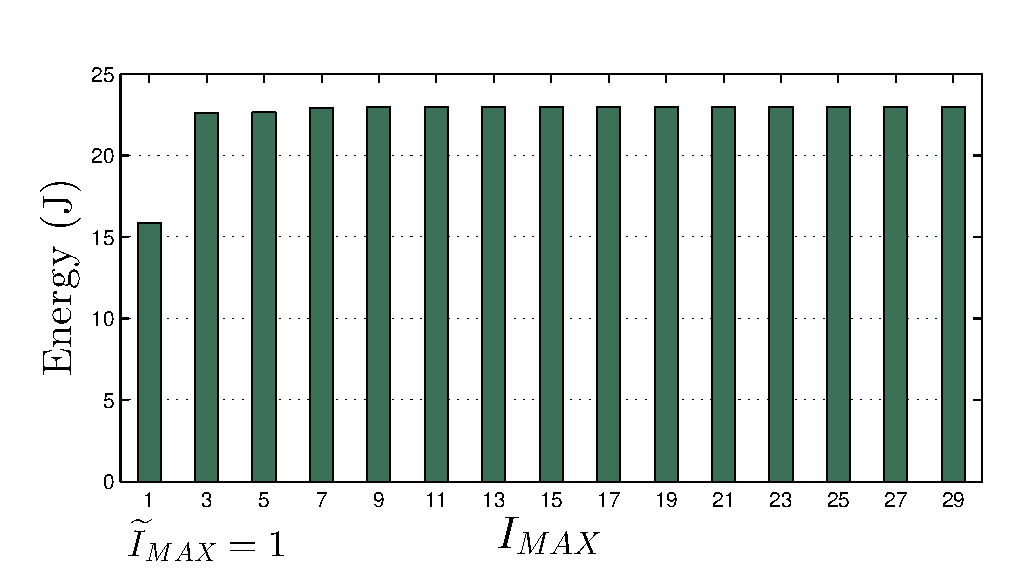
\includegraphics[width=0.9\columnwidth]{images/Fig4a} \\
     	%\label{fig:3a}
     	\vspace{10pt}
     	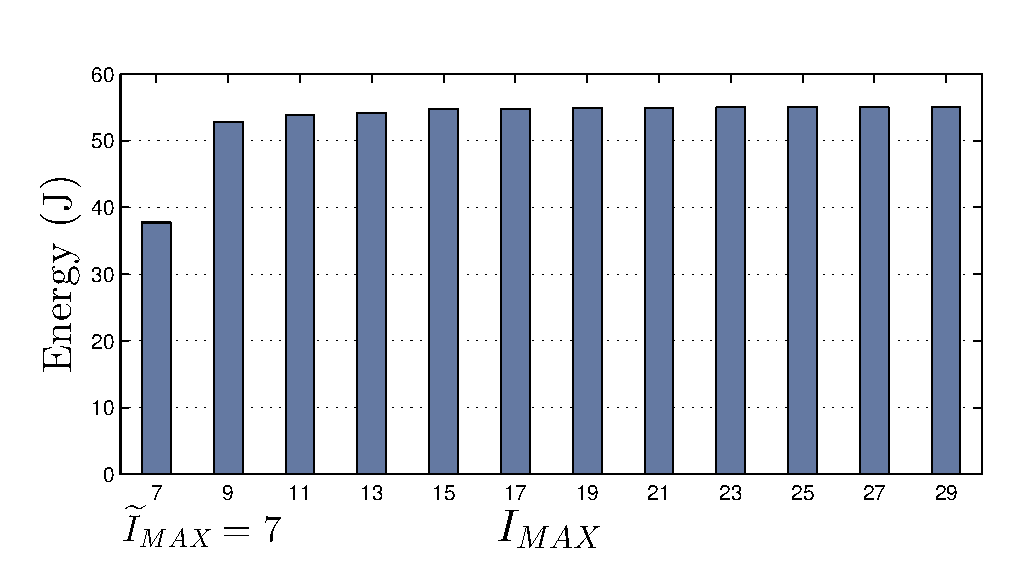
\includegraphics[width=0.9\columnwidth]{images/Fig4b}
     	\end{tikzfigure}
     	\end{minipage}
     	\begin{minipage}[t]{0.5 \linewidth}
     	\begin{tikzfigure}[...]
     	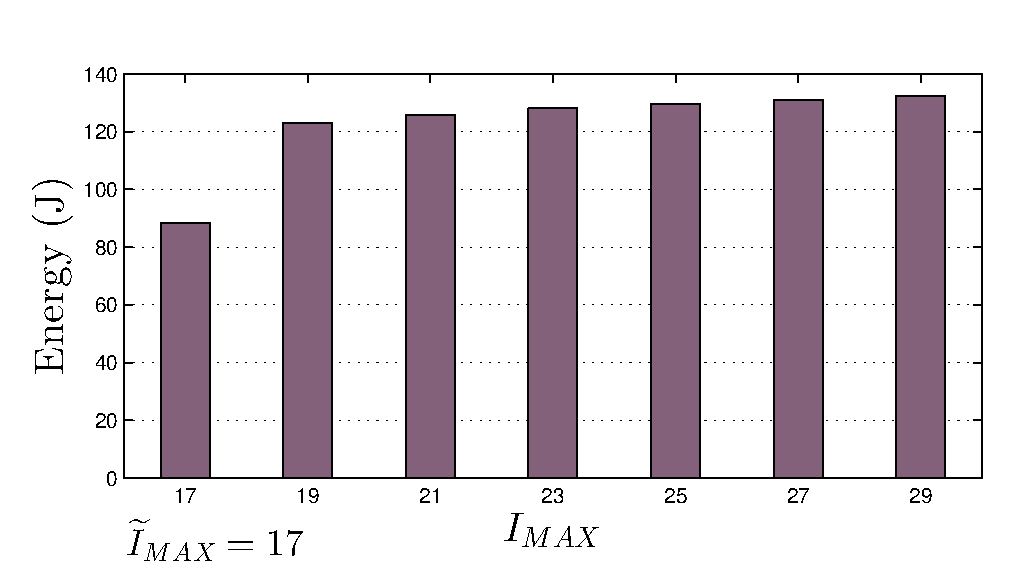
\includegraphics[width=0.9\columnwidth]{images/Fig4c}\label{fig:4}
     	\end{tikzfigure}
     	\end{minipage}
     }
     
  %%%%%%%%%% ------------------------------------------ %%%%%%%%%%
%  \blocknode%
%  {Feasibility issues and optimal scheduling}%
%  {
%  	%\begin{thm3}\label{prop:feas}
%  	\vspace{-30pt}
%  		\begin{minipage}[]{0.3\linewidth}
%  		\flushleft
%		The following inequality:\\
%		\vspace{1pt}$\:$
%  		\end{minipage}
%  		\begin{minipage}[b]{0.70 \linewidth}
%		\begin{align}\label{eq:feas}
%		\small L_t\leq\min\left\{\sum_{i=1}^{M}f_i^{\max}\Delta(i);\frac{C_{max}}{2}\left(T_t-\Delta_{max}\right)\right\},
%		\end{align}
%  		\end{minipage}
%  		%
%%  	\begin{align}\label{eq:feas}
%%  	\small
%%  	&\textbf{The following inequality:}& L_t\leq\min\left\{\sum_{i=1}^{M}f_i^{\max}\Delta(i);\frac{C_{max}}{2}\left(T_t-\Delta_{max}\right)\right\},&
%%  	\end{align}
%  	is necessary and sufficient condition for the feasibility of the constrained optimization problem
%  	in \textit{COP}.
%  	%\end{thm3}
%
%	
%	%\begin{thm3}\label{prop:opt-scheduler}
%	Let the constrained optimization problem in \textit{COP} be feasible. Thus, its solution equates (Case of quadratic energy consumption function).
%	
%	As already pointed, the form assumed by $\Phi(\eta)$ for DVFS-based CMOS CPUs is generally well approximate by quadratic one. In this case, for the optimum rate we have the following simple expression:
%	
%	\begin{minipage}[b]{0.55 \linewidth}
%		\flushleft
%		\begin{align}\label{eq:fopt-quad}	f_i^*=\left[\gamma_if_i^0+\delta_i[\mu^*-2P_i^{net}/C_{max}]_+\right]_{f_i^{min}}^{f_i^{max}},
%		\end{align}
%	\end{minipage}
%	\begin{minipage}[b]{0.40 \linewidth}
%		\begin{subequations}\label{eq:controllers}
%		\small
%		\renewcommand{\theequation}{\theparentequation.\arabic{equation}}
%		\begin{align}
%		% &\label{eq:fopt}f_i^*=\left[\pi_i^{-1}\left(2k_ef_i^0+[\mu^*-2P_i^{net}/C_{max}]_+\Delta(i)\right)\right]_{0}^{f_i^{max}}\\
%		&\label{eq:Lopt}L_i^*=\bold{1}_{[\mu^*>2P_i^{net}/C_{max}]}\left(f_i^*\Delta(i)\right),\\
%		&\label{eq:Copt}C_i^*=C_{max}\bold{1}_{[L_i^*>0]}.
%		\end{align}
%		\end{subequations}
%	\end{minipage}
%	
%
%	where $\gamma_i$ and $\delta_i$ are given by:
%	\begin{equation}
%	\label{eq:soglia_1}\gamma_i\triangleq\frac{2k_e}{2k_e+2\mathcal{E}_i^{max}/(f_i^{max})^2},\;\; \delta_i\triangleq\frac{\Delta(i)}{2k_e+2\mathcal{E}_i^{max}/(f_i^{max})^2}.
%	\end{equation}
%
%	%\footnote{$[x]_a^b$ indicates $\min\{\max\{x;a\};b\}$, while  $\textbf{1}_{[A]}$ is the (binary-valued) indicator function of the  $A$  event.}:
%	
%	The scalar $\mu^*\in\mathbb{R}_0^+$ in $f_i^*$ plays the role of a Lagrange multiplier and it is computable as the solution of the following algebraic equation:
%	$
%	\sum_{i=1}^ML_i(\mu)=L_t.
%	$
%	%\end{thm3}
%    % 
%    The optimal scheduler hibernates VM$(i)$ when the following \emph{hibernation condition} is met (see Fig. \ref{fig:2}):
%     \begin{equation}\label{eq:hib-cond}
%     \mu^*<2P_i^{net}/C_{max},\,i=1,\ldots,M.
%     \end{equation}
%  }

  
  %%%%%%%%%% ------------------------------------------ %%%%%%%%%%
%  \blocknode{Average energy consuption under random workload}%
%  {
%%  	For the heterogeneous network scenario already considered in Fig.\ref{fig:3} reports the \emph{average} energy consumptions of the optimal scheduler when the submitted workload is \emph{randomly} time-varying, that is, when the size $L_t$ of the job submitted at the beginning of each $T_t$-long round time is the outcome of a random variable (r.v.) evenly distributed over the interval $6$ - $10$ $(Mbit)$. Specifically, at the first round of the carried out simulations, all the source frequencies  $f_i^0$  in \eqref{eq:obiettivo} are reset. Afterwards, at the  $k$-th round, each $f_i^0$ is set to the corresponding optimal value $f_i^*$  already computed at the previous  $(k-1)$-th round.
%  	%For each $M$, each operative setting runs on $50000$ rounds and, then, all the reported numerical data are averaged or more than $100$ instances, so as to guarantee that each simulated point retains $95\%$ confidence interval with at least a $10\%$ precision degree.
%The plots of Fig.\ref{fig:3} may be considered representative of application scenarios where the energy due to frequency switching energy overhead is low (e.g., $k_e=0.005$ $Joule/(MHz)^2$), medium (e.g., $k_e=0.05$ $Joule/(MHz)^2$) and high (e.g., $k_e=0.5$ $Joule/(MHz)^2$). Interestingly, these plots show that: \emph{i)} the average energy consumption (quickly) increases for increasing $k_e$'s; and, \emph{ii)} the optimal number $M^*$ of VMs to be instantiated decreases for growing $k_e$'s.
%
%%Furthermore, it is worthwhile to note that the average energy consumptions of Fig.\ref{fig:3} are of about $50\%$ less than the corresponding ones previously reported in Fig.\ref{fig:2} for the case of time-invariant deterministic job sizes $L_t$'s. This is, indeed, a further consequence of the hibernation phenomena. 
%The plots of Fig.\ref{fig:4} reports the optimal allocations of the processing rates at the $1$\emph{th} round (red bars) and at the $10$\emph{th} round (blue bars) for the aforementioned heterogeneous networking case of Fig.\ref{fig:2}. The trend emerging from the plots of Fig.\ref{fig:4} is that, round-by-round, some of VMs tend to be consolidated and permanently loaded, while the remaining ones gracefully pass from the hibernation state to the off one.
%
%	\vspace{-35pt}
%	\begin{minipage}[t]{0.5 \linewidth}
%	%\flushleft
%	\begin{tikzfigure}[Average energy consumption of the optimal scheduler in the presence of randomly time-varying workload.]
%	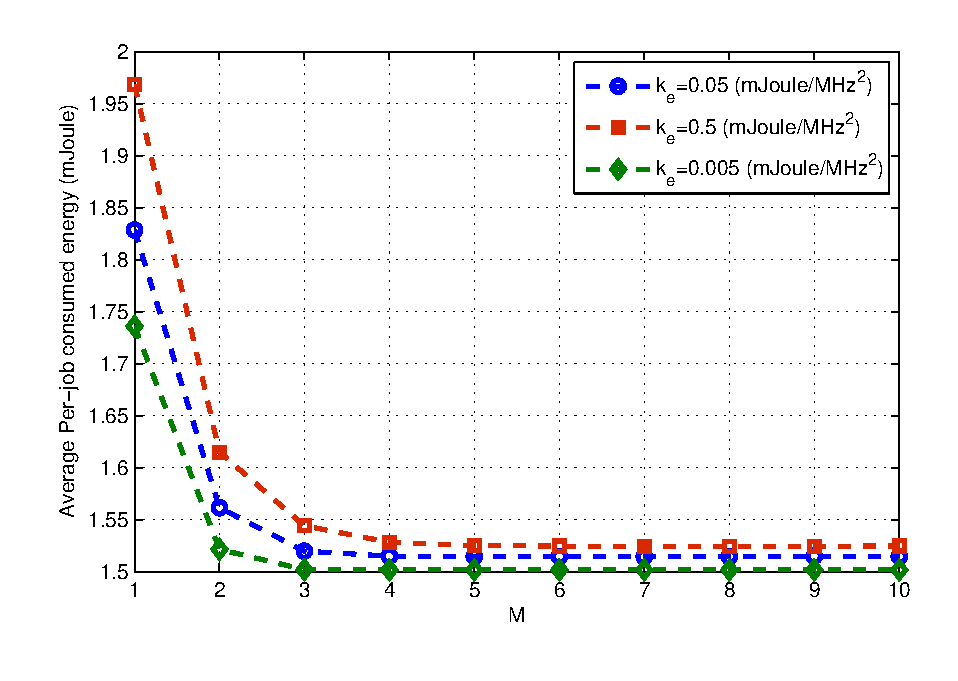
\includegraphics[height=11.5cm]{images/Cost-Tot-L-random-width2.eps}
%	\vspace{-20pt}
%	\label{fig:3aaa}
%	\end{tikzfigure}
%	\end{minipage}
%	\begin{minipage}[t]{0.45 \linewidth}
%	\begin{tikzfigure}[Allocation of the processing rates at the $1$\emph{th} round (red bars) and $10$\emph{th} round (blue bars).]
%	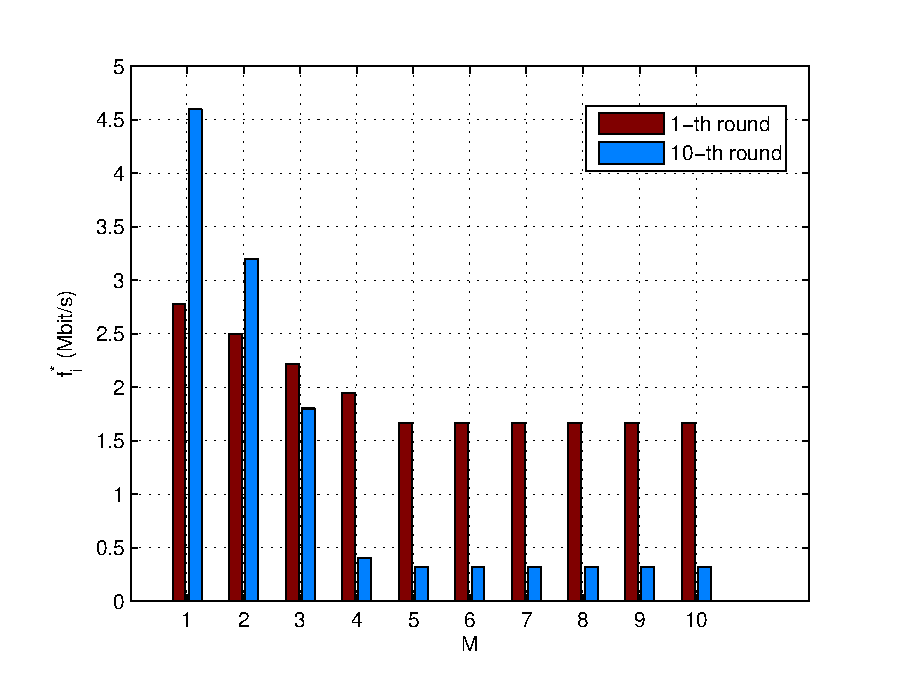
\includegraphics[height=11.5cm]{images/One-Ten-Rounds}
%	\vspace{-20pt}
%	\label{fig:4}
%	\end{tikzfigure}
%	\end{minipage}
%      
%%    \begin{tabular}[t]{ll}
%%      \begin{minipage}{0.5\linewidth}
%%        \innerblock{Theorem} {Statement}
%%      \end{minipage}
%%      & 
%%      \textbackslash innerblock\{Theorem\}\{Statement\}\\
%%
%%      \begin{minipage}{0.5\linewidth}
%%        \innerblockplain[colorone!80!]{Text}
%%      \end{minipage}
%%      &
%%      \textbackslash innerblockplain[colorone!80!]\{Text\}\\ 
%%
%%      \begin{minipage}{0.5\linewidth}
%%        \coloredbox{colorthree!50!}{Text}
%%      \end{minipage}
%%      &
%%      \textbackslash coloredbox\{colorthree!50!\}\{Text\}
%%    \end{tabular}
%%
%%    \vspace{0.5cm}
%%    The default figure environment does not work within a tikzpicture. I created
%%    a new figure environment that can be used instead, based on the code sent by
%%    Stephan Thober.
%%    \begin{itemize}
%%    \item[] \textbackslash begin\{tikzfigure\}[Caption]\\
%%      \ldots\\
%%      \textbackslash end\{tikzfigure\}
%%    \end{itemize} 
%%    % 
%%
%%	\emph{note}
%  }
%
%
%  %% to place the next node centered vertically in the second column, we can
%  %% obtain the y-coordinate of the previous node using macro
%  %% \getcurrentrow{note}, where note is the alias of the callout node, and
%  %% then specify the coordinate of the next node using coordinate (currentrow)
%  %\getcurrentrow{note}
%	%\getcurrentrow{note}
	
  %% a plain block
  %% #1 - rotate angle (optional), #2 - where, #3 - width, #4 - title, #5 - text
  %%%%%%%%%% ------------------------------------------ %%%%%%%%%%
  \plainblock{($(currenty)$)} %-(xshift) + (xshift) -(yshift) %[($(currenty)+(0,10)$)]%
  {38}{Conclusion} %
  {
  	We developed the optimal bandwidth manager for intra-datacenter live VM migration. It minimizes at run-time the communication energy wasted by the migration of the VM memory under hard QoS constraints on both the migration time and downtime. After implementing it atop a wired test-bed, we measured and compared its energy performance by considering synthetic and real-world workloads, as well as random and ordered migration scheduling disciplines. The carried out field trials highlight that the average energy saving of the proposed bandwidth manager over the corresponding state-of-the-art Xen one is over 40\% and approaches 66\% under strict constraints on the tolerated downtimes. Interestingly, the measured per-migration CPU slow-down induced by its implementation is, in average, limited up to 1.5${-}$2\%, while the measured average stretching of the execution times of the migrated applications is under 20\%.
  	
%  	Regarding hints for future research, we point out that the reported BMOP formulation of Eqs. \eqref{eqn_18.1}, \eqref{eqn_18.2} may apply verbatim to live VM migration over WAN connections, provided that the adopted power-rate function in \eqref{eqn_8}, setup energy in \eqref{eqn_11} and round-trip-time in \eqref{eqn_9} are suitable modeled. In fact, we stress that, from a networking perspective, guaranteeing seamless migration of IP-addressed VMs over WANs poses quite specific challenges. First, in NAS-equipped LAN environments, it suffices that, during the stop-and-copy phase, the destination server broadcasts an  unsolicited ARP reply message, in order to advertise all the LAN interfaces that the IP address of the migrated VM has been moved to a new server. However, more challenging is to attain seamless traffic redirection when the VM migrates over different subnets \cite{6-Mishra}.

%    \begin{itemize}
%    \item[] \textbackslash plainblock[rotate angle]\{coordinate\}\{Block Width\}\{Block
%      Title\}\{Block Content\} 
%    \end{itemize}
  }
  
  %% the coordinate (currenty) is used in the default placing of the next blocknode
 



   %%%%%%%%%%%%% NEW COLUMN %%%%%%%%%%%%%%% 
  %% (if column number is 3)
  \startthirdcolumn

  %%%%%%%%%% ------------------------------------------ %%%%%%%%%%
%  \blocknode {Personalizing the Poster}%
%  {It is possible to adjust the layout of the poster. To impose your own
%    setting, you can use these macros:
%    \begin{itemize}
%    \item Macros for changing sizes
%      \begin{itemize}
%      \item[] \textbackslash setmargin\{4\},
%        %% the height of the head drawing on top
%        %% applicable to templates N2 and 4
%        \textbackslash setheaddrawingheight\{14\},
%        %% the space between two or more groups of authors from different
%        %% institutions
%        %% used in \maketitle
%        \textbackslash setinstituteshift\{10\},\\
%        %% the space between the blocks
%        %% default value is 2cm
%        \textbackslash setblockspacing\{2\},
%        %% the height of the title stripe in block nodes, decrease it to save space
%        %% default value is 3cm
%        \textbackslash setblocktitleheight\{3\}
%      \end{itemize}
%
%    \item Other structural macros
%      \begin{itemize}
%      \item[]  %% the number of columns in the poster, possible values 2,3
%        %% default value is 2
%        \textbackslash setcolumnnumber\{3\},
%        %% which template to use 
%        %% N1 simple, standard look, with a colored background and gray boxes
%        %% N2 board with nodes
%        %% N3 another standard look
%        %% N4 envelope like look
%        %% N5 with a wave-like head, original idea taken from
%        %%%% http://fc09.deviantart.net/fs71/f/2010/322/1/1/scientific_poster_by_nabuy-d333ria.jpg
%        %% N6 experimental, oriental style, largely based on template N3
%        \textbackslash usetemplate\{6\},\\
%        \textbackslash usecolortemplate\{4\},
%        \textbackslash usebackgroundtemplate\{5\},
%        \textbackslash usetitletemplate\{2\},\\
%        \textbackslash useblocknodetemplate\{5\},
%        \textbackslash useinnerblocktemplate\{3\},
%        \textbackslash useplainblocktemplate\{4\}
%
%      \end{itemize}
%
%    \item Macro for adding logos to the title block
%      \begin{itemize}
%      \item[] \textbackslash addlogo[south west]\{(0,0)\}\{6cm\}\{filename\}
%      \end{itemize}
%
%    \item Macros for the basic colors
%      \begin{itemize}
%      \item[] \textbackslash setfirstcolor\{green!70!\}, % default 116699
%        \textbackslash setsecondcolor\{gray!80!\}, % default CCCCCC
%        \textbackslash setthirdcolor\{red!80!black\}% default 991111
%      \end{itemize}
%
%    \item Macros for specific colors:
%      \begin{itemize}
%      \item[] \textbackslash setbackgrounddarkcolor\{colorone!70!black\},
%        \textbackslash setbackgroundlightcolor\{{\small colorone!70!}\},\\
%        \textbackslash settitletextcolor\{textcolor\},
%        \textbackslash settitlefillcolor\{white\},
%        \textbackslash settitledrawcolor\{colortwo\},\\
%        \textbackslash setblocktextcolor\{textcolor\},
%        \textbackslash setblockfillcolor\{white\},\\
%        \textbackslash setblocktitletextcolor\{colorone\},
%        \textbackslash setblocktitlefillcolor\{colortwo\}, \\
%        \textbackslash setplainblocktextcolor\{textcolor\},
%        \textbackslash setplainblockfillcolor\{colorthree!40\},\\
%        \textbackslash setplainblocktitletextcolor\{textcolor\},
%        \textbackslash setplainblocktitlefillcolor\{colorthree!60\}, \\
%        \textbackslash setinnerblocktextcolor\{textcolor\},
%        \textbackslash setinnerblockfillcolor\{white\},\\
%        \textbackslash setinnerblocktitletextcolor\{white\},
%        \textbackslash setinnerblocktitlefillcolor\{colorthree\},
%      \end{itemize}
%    \end{itemize}
%  }



\end{tikzpicture}


\end{document}




